\documentclass[]{beamer}

% Font encoding and input
\usepackage[T1]{fontenc}
\usepackage[utf8]{inputenc}
\usepackage{microtype}

% Core packages
\usepackage{graphicx}
\usepackage{url}
\usepackage{listings}
\usepackage{booktabs}
\usepackage{xcolor}
\usepackage{amsmath}
\usepackage{amsfonts}
\usepackage{amssymb}

\usepackage[spanish]{babel} %use your language

\setbeamertemplate{bibliography item}[text]

\usetheme{UTN-BHI}

% Add a section slide.
% Remove it if you prefer that option.
% \AtBeginSection[]{
%   \begin{frame}
%   \vfill
%   \centering
%   \begin{beamercolorbox}[sep=8pt,center]{title}
%     \usebeamerfont{title}\insertsectionhead\par%
%   \end{beamercolorbox}
%   \vfill
%   \end{frame}
% }

% Enhanced code style
\lstdefinestyle{myC++Style}{
  language=C++,
  basicstyle=\ttfamily\small,
  keywordstyle=\color{blue}\bfseries,
  commentstyle=\color{green!60!black},
  stringstyle=\color{red},
  numberstyle=\tiny\color{gray},
  showspaces=false,
  showstringspaces=false,
  breaklines=true,
  numbers=left,
  frame=single,
  backgroundcolor=\color{gray!10},
  captionpos=b
}

\urldef{\email}\path|jiparraguirre@frbb.utn.edu.ar|
\title[]{La Evolución de un Clásico: Un Proyecto de Pong en Tres Partes}
\subtitle{De la Consola a los Gráficos en C}

\author[J. Iparraguirre] {Javier Iparraguirre}

\institute{
Universidad Tecnológica Nacional\\
11 de abril 461, Bahía Blanca, Argentina\\
\email\\
\url{http://www.frbb.utn.edu.ar/}}

\date{\today}

\begin{document}

\begin{frame}
  \titlepage
\end{frame}

\section{Resumen del Proyecto}

\begin{frame}
  \frametitle{Pong}
  \begin{figure}
    \centering
    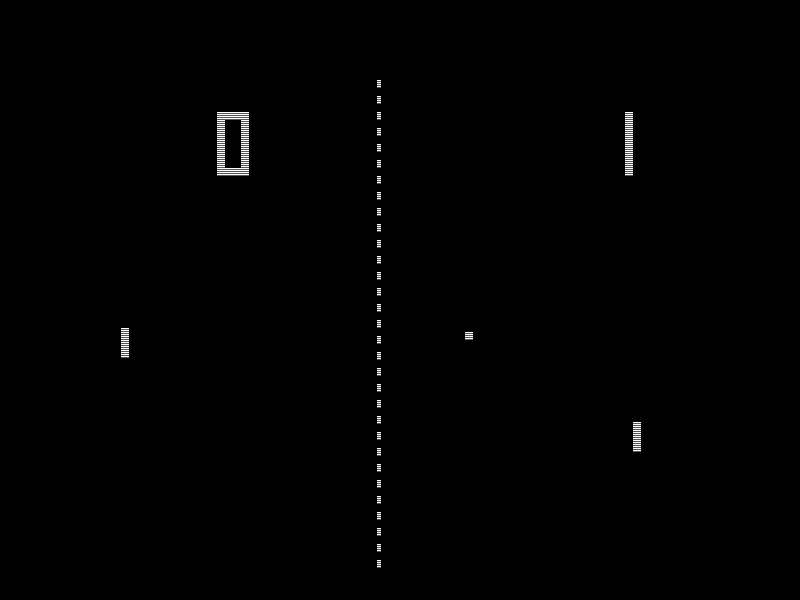
\includegraphics[width=0.7\textwidth]{figures/Pong.png}
    \caption{Juego clásico de Pong}
  \end{figure}
\end{frame}

\begin{frame}
  \frametitle{Pong}
  \begin{figure}
    \centering
    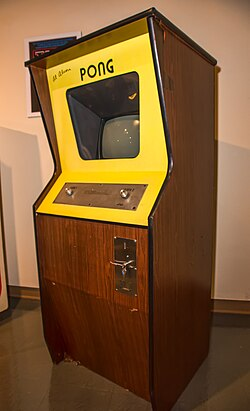
\includegraphics[width=0.38\textwidth]{figures/Signed_Pong_Cabinet.jpg}
  \end{figure}
\end{frame}


\begin{frame}
  \frametitle{Resumen del Proyecto}
  \begin{itemize}
    \item Esta presentación explora tres implementaciones del clásico juego Pong \cite{wikipedia_pong}, cada una demostrando un nivel diferente de complejidad en la programación.
    \item Viajaremos desde una simple aplicación de consola multiplataforma, pasando por una versión con una estructura de proyecto profesional, hasta llegar a un juego gráfico completo usando la librería SDL3.
  \end{itemize}
\end{frame}

\section{Implementación 1: La Base - Pong en Consola}
\begin{frame}
  \frametitle{Implementación 1: La Base - Pong en Consola}
  \subtitle{\texttt{01-simple}: C Puro, Multiplataforma}
  \begin{itemize}
    \item \textbf{Tecnología:} Escrito completamente en C estándar \cite{pong_simple}.
    \item \textbf{Multiplataforma:} Compatible con Windows, Linux, y macOS \cite{pong_simple}.
    \item \textbf{Gráficos:} Utiliza caracteres ASCII y códigos de escape ANSI para renderizar en la terminal \cite{pong_simple}.
    \item \textbf{Jugabilidad:} Un juego funcional de Jugador vs. IA de Pong.
  \end{itemize}
\end{frame}

\begin{frame}[fragile]
    \frametitle{Implementación 1: Fragmento de Código}
    \lstset{style=myC++Style, language=C}
    \begin{lstlisting}[]
// Dibuja todo el juego
void draw_game(void)
{
    int i, j;

    gotoxy(0, 0);

    // Dibuja el borde superior
    for (i = 0; i < FIELD_WIDTH; i++)
    {
        printf("#");
    }
    printf("\n");

    // ... (resto de la logica de dibujo)
}
    \end{lstlisting}
\end{frame}

\section{Implementación 2: Estructura Profesional - Proyecto de Visual Studio}
\begin{frame}
  \frametitle{Implementación 2: Estructura Profesional}
  \subtitle{\texttt{02-simple-visual-studio}: Organizado para el Desarrollo}
  \begin{itemize}
    \item \textbf{Mejoras:} Construido sobre la primera implementación.
    \item \textbf{Entorno de Desarrollo:} Incluye un proyecto completo de Visual Studio (\texttt{.vcxproj}, \texttt{.sln}) \cite{pong_vs_project, pong_vs_solution}.
    \item \textbf{Código Base:} El mismo código C multiplataforma, pero ahora estructurado para un IDE profesional \cite{pong_vs_main}.
  \end{itemize}
\end{frame}

\begin{frame}
  \frametitle{Implementación 2: ¿Por qué Visual Studio?}
  \begin{itemize}
    \item \textbf{Depuración:} Herramientas de depuración avanzadas para recorrer el código e inspeccionar variables.
    \item \textbf{Gestión de Proyectos:} Simplifica la gestión de archivos fuente, dependencias y configuraciones de compilación.
    \item \textbf{IntelliSense:} Completado de código y características de navegación mejoradas.
  \end{itemize}
\end{frame}

\section{Implementación 3: El Salto a Gráficos - SDL3}
\begin{frame}
  \frametitle{Implementación 3: El Salto a Gráficos - SDL3}
  \subtitle{\texttt{03-simple-visual-studio-sdl}: Un Enfoque Moderno}
  \begin{itemize}
    \item \textbf{Lenguaje:} C.
    \item \textbf{Librería Gráfica:} Utiliza la potente librería SDL3 para renderizado 2D.
    \item \textbf{Visuales:} Gráficos fluidos y acelerados por hardware reemplazan la interfaz ASCII.
    \item \textbf{Características Avanzadas:} Introduce conceptos más complejos como sistemas de tiempo real y una IA mejorada.
  \end{itemize}
\end{frame}

{
\usebackgroundtemplate{\includegraphics[width=\paperwidth]{theme/utn-bhi-page-blank.png}}
\begin{frame}[fragile]
  \frametitle{Implementación 3: Avances Técnicos}
  \begin{itemize}
    \item \textbf{Principios Orientados a Estructuras:} El juego se estructura en torno a \texttt{GameObject} y \texttt{GameState} \cite{pong_sdl_main}.
    \item \textbf{Programación Orientada a Eventos:} El bucle del juego ahora es impulsado por eventos de SDL para la entrada y gestión de la ventana \cite{pong_sdl_main}.
    \item \textbf{Renderizado:} El renderizador de SDL se utiliza para dibujar formas y gestionar la ventana del juego \cite{pong_sdl_main}.
    \item \textbf{IA:} La IA es más receptiva e inteligente, con su propia lógica de actualización \cite{pong_sdl_main}.
  \end{itemize}
  \lstset{style=myC++Style}
  \begin{lstlisting}[]
// Esta funcion se ejecuta una vez por frame,
// y es el corazon del programa.
SDL_AppResult SDL_AppIterate(void *appstate)
{
    // ... (logica del juego y renderizado)
}
  \end{lstlisting}
\end{frame}
}

\section{Comparando las Implementaciones}
\begin{frame}
  \frametitle{Comparando las Implementaciones}
  \tiny{
  \begin{table}
  \centering
  \begin{tabular}{@{}p{2.2cm}p{1.8cm}p{1.8cm}p{2.2cm}@{}}
  \toprule
  \textbf{Característica} & \textbf{01-simple} & \textbf{02-simple-vs} & \textbf{03-simple-sdl} \\
  \midrule
  Lenguaje & C & C & C \\
  Gráficos & ASCII & ASCII & SDL3 \\
  Plataforma & Multi-plataforma & Multi-plataforma & Windows (Config.) \\
  Desarrollo & Editor Básico & Visual Studio & Visual Studio \\
  Complejidad & Baja & Media & Alta \\
  \bottomrule
  \end{tabular}
  \caption{Una comparación lado a lado}
  \end{table}
  }
\end{frame}

\section{Progresión del Aprendizaje}
\begin{frame}
  \frametitle{Progresión del Aprendizaje}
  \begin{itemize}
    \item \textbf{\texttt{01-simple}:} Domina los fundamentos de la programación en C y el desarrollo multiplataforma.
    \item \textbf{\texttt{02-simple-visual-studio}:} Aprende prácticas de desarrollo profesional y los beneficios de un IDE.
    \item \textbf{\texttt{03-simple-visual-studio-sdl}:} Introduce el mundo de la programación gráfica y el desarrollo de juegos.
  \end{itemize}
\end{frame}

\section{Conclusión}
\begin{frame}
  \begin{center}
    \begin{beamercolorbox}[sep=8pt,center]{title}
      \Large{¡Gracias!}
    \end{beamercolorbox}
    \vspace{1em}
    \huge{¿Preguntas?}\\
    \vspace{1em}
    \small{\email}

  \end{center}
\end{frame}

{
\usebackgroundtemplate{\includegraphics[width=\paperwidth]{theme/utn-bhi-page-blank.png}}
\section{Referencias}
\begin{frame}[allowframebreaks]
  \frametitle{Referencias}
  \bibliographystyle{alpha}
  \bibliography{references}
\end{frame}
}

\end{document}
